\documentclass[11pt,a4paper]{article}

% Image mode: pdf.
% Image paths stay relative. In PDF mode, place same-basename PDF conversions
% of the chapter SVG files in the assets/ directory beside this source.

\usepackage{iftex}
\ifPDFTeX
  \PackageError{handout}{This template requires XeTeX or Tectonic}{Compile with xelatex or tectonic.}
\fi

\usepackage[a4paper,top=18mm,bottom=20mm,left=20mm,right=20mm,headsep=6mm]{geometry}
\usepackage{fontspec}
\usepackage{xeCJK}
\usepackage{amsmath}
\usepackage{unicode-math}

% Font settings are intentionally visible in the generated .tex file.
% These defaults target the macOS machine used for the released PDF.
% Change the family names when compiling on another system.
\setmainfont{Songti TC}
\setsansfont{Heiti TC}
\setmonofont{Menlo}
\setCJKmainfont{Songti TC}
\setCJKsansfont{Heiti TC}
\setCJKmonofont{Heiti TC}
\setmathfont{STIX Two Math}
\XeTeXlinebreaklocale "zh"
\XeTeXlinebreakskip=0pt plus 1pt

\usepackage{xcolor}
\definecolor{HandoutBlue}{HTML}{215A91}
\definecolor{HandoutBlueLight}{HTML}{EEF5FC}
\definecolor{HandoutGreen}{HTML}{39715A}
\definecolor{HandoutGreenLight}{HTML}{EFF8F3}
\definecolor{HandoutGold}{HTML}{8A641C}
\definecolor{HandoutGoldLight}{HTML}{FFF8E8}
\definecolor{HandoutInk}{HTML}{253142}
\definecolor{HandoutMuted}{HTML}{667085}

\usepackage{graphicx}
\makeatletter
% Pandoc 3 emits an accessibility `alt` key for raster/PDF images. Older
% graphicx releases do not know that key, so accept it without changing layout.
\@ifundefined{KV@Gin@alt}{\define@key{Gin}{alt}{}}{}
\newsavebox\pandoc@box
\newcommand*\pandocbounded[1]{%
  \sbox\pandoc@box{#1}%
  \Gscale@div\@tempa{\textheight}{\dimexpr\ht\pandoc@box+\dp\pandoc@box\relax}%
  \Gscale@div\@tempb{\linewidth}{\wd\pandoc@box}%
  \ifdim\@tempb\p@<\@tempa\p@\let\@tempa\@tempb\fi
  \ifdim\@tempa\p@<\p@\scalebox{\@tempa}{\usebox\pandoc@box}%
  \else\usebox{\pandoc@box}%
  \fi
}
\makeatother
\usepackage{float}
\floatplacement{figure}{H}
% Pandoc uses LTcaptype=none for uncaptioned longtables. The caption package
% expects that name to exist as a counter even though it is never displayed.
\newcounter{none}
\usepackage{caption}
\captionsetup[figure]{labelformat=empty,labelsep=none,font=small}

\usepackage{booktabs,longtable,array,calc}
\usepackage{etoolbox}
\makeatletter
\patchcmd\longtable{\par}{\if@noskipsec\mbox{}\fi\par}{}{}
\makeatother

\usepackage[most]{tcolorbox}
\tcbuselibrary{breakable,skins}
\newtcolorbox{HandoutLearningMap}{
  enhanced,breakable,colback=HandoutBlueLight,colframe=HandoutBlue,
  boxrule=0.8pt,arc=1.5mm,left=3mm,right=3mm,top=2mm,bottom=2mm,
  before skip=8pt,after skip=10pt
}
\newtcolorbox{HandoutWorkedExample}{
  enhanced,breakable,colback=HandoutGreenLight,colframe=HandoutGreen,
  boxrule=0.65pt,arc=1.5mm,left=3mm,right=3mm,top=2mm,bottom=2mm,
  before skip=8pt,after skip=10pt
}
\newtcolorbox{HandoutSelfCheck}{
  enhanced,breakable,colback=HandoutGoldLight,colframe=HandoutGold,
  boxrule=0.65pt,arc=1.5mm,left=3mm,right=3mm,top=2mm,bottom=2mm,
  before skip=8pt,after skip=10pt
}

\usepackage{titlesec}
\titleformat{\section}{\sffamily\bfseries\Large\color{HandoutBlue}}{}{0pt}{}
\titleformat{\subsection}{\sffamily\bfseries\large\color{HandoutInk}}{}{0pt}{}
\titleformat{\subsubsection}{\sffamily\bfseries\normalsize\color{HandoutInk}}{}{0pt}{}
\titlespacing*{\section}{0pt}{1.4em}{0.55em}
\titlespacing*{\subsection}{0pt}{1.15em}{0.45em}
\titlespacing*{\subsubsection}{0pt}{0.9em}{0.35em}
\setcounter{secnumdepth}{-\maxdimen}

\usepackage{hyperref}
\usepackage{bookmark}
\IfFileExists{xurl.sty}{\usepackage{xurl}}{}
\urlstyle{same}
\hypersetup{
  colorlinks=true,
  linkcolor=HandoutBlue,
  urlcolor=HandoutBlue,
  citecolor=HandoutBlue,
  pdftitle={必物-1 科學的態度與方法},
  pdfsubject={物理},
  pdfcreator={Pandoc with the HighSchooContent LaTeX template}
}

\setlength{\parindent}{0pt}
\setlength{\parskip}{0.55em plus 0.15em minus 0.1em}
\setlength{\emergencystretch}{3em}
\setlength{\LTpre}{0.5em}
\setlength{\LTpost}{0.5em}
\renewcommand{\arraystretch}{1.18}
\providecommand{\tightlist}{%
  \setlength{\itemsep}{0pt}\setlength{\parskip}{0pt}}
\pagestyle{plain}


\begin{document}

\begin{tcolorbox}[
  enhanced,colback=white,colframe=HandoutBlue,boxrule=1.1pt,arc=2mm,
  borderline west={3pt}{0pt}{HandoutBlue},left=5mm,right=4mm,top=4mm,bottom=4mm
]
{\sffamily\small\bfseries\color{HandoutBlue}學生講義}\par
{\sffamily\bfseries\LARGE\color{HandoutInk}必物-1 科學的態度與方法}\par
\vspace{0.35em}{\large 從可檢驗主張、量測資料與共同單位，建立能預測且可重複檢查的物理模型}\par
\vspace{0.45em}{\small\color{HandoutMuted}%
科目：物理
\quad 課程：普通高中必修物理
\quad 版本：學生版｜核心＋理解
\quad 校訂：2026-08-29
}\par
\vspace{0.25em}{\small\color{HandoutMuted}範圍：科學態度、科學方法、物理量與國際單位制、前綴與數量級、物理學範疇及發展}\par
\end{tcolorbox}


物理學把自然現象轉成可量測的物理量，從資料尋找數學關係，再用模型預測尚未量過的情況。可信的結論必須交代測量方式、單位、控制條件、原始資料與模型適用範圍，讓其他人能依同一程序重複檢查。本章建立這套共同語言，也說明力學、熱學、電磁學、光學與近代物理如何由觀測、實驗與數學模型逐步發展。

\begin{HandoutLearningMap}

\subsection{本章問題與能力}\label{ux672cux7ae0ux554fux984cux8207ux80fdux529b}

\begin{enumerate}
\def\labelenumi{\arabic{enumi}.}
\tightlist
\item
  如何把一段說法改寫成能由觀測結果支持或修正的科學主張？
\item
  如何區分觀察、假設、預測與結論，並用控制變因及重複量測建立資料？
\item
  如何使用 SI 基本單位、導出單位、前綴詞與數量級，使量測能跨實驗室比較？
\item
  如何依現象與條件選擇物理領域和模型，並從物理史辨認證據、預測與統一的關係？
\end{enumerate}

\subsection{實際用途}\label{ux5be6ux969bux7528ux9014}

實驗設計可檢查產品、藥物與環境資料；共同單位保障工程製造、醫療校正與國際合作；數量級能快速檢查答案；模型條件則決定日常力學、半導體量子模型或相對論何時適用。

\end{HandoutLearningMap}

{\def\LTcaptype{none} % do not increment counter
\begin{longtable}[]{@{}lll@{}}
\toprule\noalign{}
工作 & 必須留下的資訊 & 可回答的問題 \\
\midrule\noalign{}
\endhead
\bottomrule\noalign{}
\endlastfoot
提出假設 & 可觀測的預測、適用條件 & 哪一種結果支持或削弱假設？ \\
設計實驗 & 自變量、應變量、控制變因、操作方式 & 比較是否公平？ \\
報告測量 & 數值、單位、原始資料與處理方法 & 他人能否重複？ \\
建立模型 & 數學關係、誤差大小、適用範圍 & 新條件下會發生什麼？ \\
選擇理論 & 尺度、速度、重力與研究對象 & 使用古典或近代模型？ \\
\end{longtable}
}

\section{1　科學的態度}\label{ux79d1ux5b78ux7684ux614bux5ea6}

\subsection{1.1 可檢驗性與證據}\label{ux53efux6aa2ux9a57ux6027ux8207ux8b49ux64da}

科學研究物質世界中可觀測、可量測或可由觀測間接推論的現象。科學主張必須具有可檢驗性：它要能導出具體預測，而且可能的觀測結果能區分「預測得到支持」與「假設需要修正」。

例如「固定斜面與球，由靜止釋放時，位移 \(s\) 與時間平方 \(t^2\) 成正比」會預測：

\[
\frac{s}{t^2}=k
\]

在量測不確定範圍內近似固定，且 \(s-t^2\) 圖接近通過原點的直線。這些預測都能由實驗檢查。

科學態度落實在下列行動：

\begin{itemize}
\tightlist
\item
  理性：把觀察到的事實、由事實作出的推論、以及個人偏好分開。
\item
  客觀：事先訂定量測方式與判準，使不同研究者能依相同規則處理資料。
\item
  誠實：完整保存原始資料、修改紀錄與排除資料的理由。
\item
  適當懷疑：同時檢查新主張、既有理論、儀器與自己的推理。
\item
  謙遜與開放：用新證據調整結論，並清楚說明目前仍未知的部分。
\item
  尊重：科學能處理可檢驗的物質世界問題；價值、藝術與信仰還包含科學量測以外的判準。
\end{itemize}

理論的可信度來自多次、跨條件、可重複的檢驗。一次符合能提高可信度；新的條件可能顯示原模型的適用界線。牛頓力學在日常低速尺度仍十分準確，而高速、強重力或原子尺度需要更廣的模型。

\begin{figure}
\centering
\pandocbounded{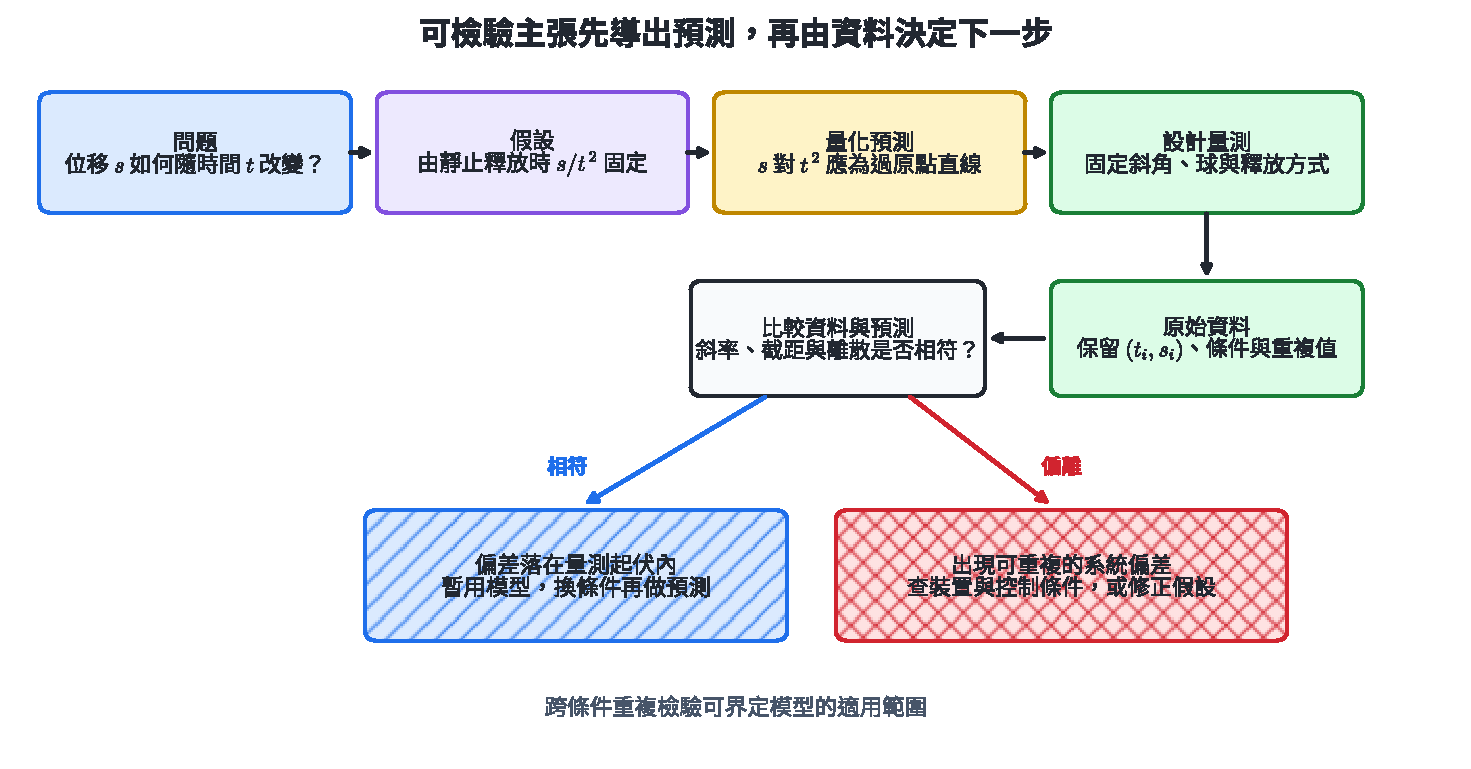
\includegraphics[keepaspectratio,alt={可檢驗主張與科學循環}]{assets/必物-1-可檢驗主張與科學循環.pdf}}
\caption{可檢驗主張與科學循環}
\end{figure}

圖 1｜假設先導出可量化預測；原始資料與預測比較後，再決定暫用模型或回查裝置、控制條件與假設。

圖中的科學方法是一個循環。問題引出假設，假設導出預測，實驗產生資料；資料與預測比較後，可建立暫時模型，也可回到裝置、量測或假設重新檢查。成熟模型還要在新條件下預測，再接受新的測試。

\subsection{1.2 觀察、推論與結論}\label{ux89c0ux5bdfux63a8ux8ad6ux8207ux7d50ux8ad6}

觀察是由感官或儀器直接得到的紀錄，例如「兩張相同紙從同高度釋放，揉成團的紙較早落地」。推論是根據觀察提出的解釋，例如「攤平紙受到較大的空氣阻力」。結論則要由能區分不同解釋的實驗支持。

同一觀察常有多個可能解釋。把紙揉成團同時改變形狀、迎風面積與氣流，因此原實驗無法單獨判斷質量是否影響落下時間。後續設計可以固定形狀與迎風面積，只改變質量；也可在低壓環境比較，以檢查空氣阻力的影響。

資料偏離理論預期時，可靠的處理順序是：

\begin{enumerate}
\def\labelenumi{\arabic{enumi}.}
\tightlist
\item
  保存原始資料與量測時間。
\item
  檢查儀器校正、操作條件、抄錄與單位。
\item
  依事先規則判斷是否有可辨認的操作失誤。
\item
  重複量測，確認偏離是否穩定出現。
\item
  依證據修正實驗、假設或模型。
\end{enumerate}

這套做法能分辨偶然起伏、系統性的儀器問題與真正的新現象。只保留接近預期的資料會破壞這項分辨能力。

\subsection{1.3 科學結論與權威}\label{ux79d1ux5b78ux7d50ux8ad6ux8207ux6b0aux5a01}

科學家的經驗能幫助提出更好的問題與設計，但姓名、職位或名望本身不構成自然現象的證據。若量測結果與教科書數值不同，研究者應先檢查程序、單位、儀器與重複性，再完整報告差異。經過獨立重複仍存在的差異，才有機會指出模型條件或新現象。

同樣地，單次實驗也很少能直接建立普遍定律。普遍結論需要不同研究者、不同儀器、不同樣本與不同條件的交叉檢驗。科學共同體的作用，是公開方法與資料，讓主張能被反覆檢查。

科學態度直接用在新聞判讀、商品宣稱、環境監測與醫療證據。讀到「使用後效果提升」時，可以追問：效果如何定義？與哪一組比較？樣本數多少？測量單位與原始資料是什麼？是否由獨立團隊重複？

\subsubsection{示範 1　把籠統說法改寫成可檢驗假設}\label{ux793aux7bc4-1-ux628aux7c60ux7d71ux8aaaux6cd5ux6539ux5bebux6210ux53efux6aa2ux9a57ux5047ux8a2d}

說法：「較重的物體落得較快。」

\begin{enumerate}
\def\labelenumi{\arabic{enumi}.}
\tightlist
\item
  指定對象：相同形狀、相同尺寸，但質量不同的兩個球。
\item
  指定條件：由同一高度同時由靜止釋放，環境風速相同。
\item
  指定觀測量：由電子計時器量落地時間。
\item
  寫成假設：「在上述條件下，質量較大的球落地時間較短。」
\item
  寫出區分結果：若不同質量的球在量測解析度內具有相同落地時間，原假設缺乏支持；若差異可重複且超過量測起伏，再檢查質量或空氣阻力模型。
\end{enumerate}

籠統說法經過對象、條件與觀測量的操作化後，才成為可檢查的主張。

\subsubsection{示範 2　處理偏離已知值的資料}\label{ux793aux7bc4-2-ux8655ux7406ux504fux96e2ux5df2ux77e5ux503cux7684ux8cc7ux6599}

學生量測基本電荷，五次結果為

\[
1.57,\ 1.61,\ 1.59,\ 2.45,\ 1.60
\quad(\times10^{-19}\ \mathrm C).
\]

第四筆明顯較大。合乎科學態度的處理為：

\begin{enumerate}
\def\labelenumi{\arabic{enumi}.}
\tightlist
\item
  五筆都保留在原始紀錄。
\item
  回查第四次的電壓檔位、液滴編號、時間讀值與換算單位。
\item
  若找到明確抄錄錯誤，例如把 \(0.245\) 寫成 \(2.45\)，保留原值與更正紀錄。
\item
  若找不到原因，增加重複次數並分別報告「含第四筆」與「依事先判準排除第四筆」的結果。
\end{enumerate}

這樣才能讓他人判斷偏離來自操作、隨機起伏或模型尚未考慮的因素。

\subsubsection{示範 3　區分觀察與解釋}\label{ux793aux7bc4-3-ux5340ux5206ux89c0ux5bdfux8207ux89e3ux91cb}

敘述甲：「接通電流後，附近磁針偏轉 \(18^\circ\)。」這是儀器觀察。

敘述乙：「電流在導線周圍產生磁效應。」這是由多次觀察建立的解釋。

敘述丙：「電流加倍時，磁針偏角也加倍。」這是可進一步檢驗的預測。要測試丙，需固定導線位置、磁針、環境磁場與量測方法，只改變電流。

\subsection{1.4 節內練習}\label{ux7bc0ux5167ux7df4ux7fd2}

\begin{enumerate}
\def\labelenumi{\arabic{enumi}.}
\tightlist
\item
  將下列兩句分成觀察與推論：「金屬棒加熱後長度增加 \(0.8\ \mathrm{mm}\)；金屬內粒子平均間距增大。」
\item
  把「亮一點的燈比較耗電」改寫成包含控制條件、觀測量與可區分結果的假設。
\item
  兩張相同紙，一張攤平、一張揉成團，揉成團者先落地。列出至少兩個同時改變的因素，並提出一個較公平的比較。
\item
  六次量測中有一筆遠離其他值。寫出三項在決定是否排除前應完成的工作。
\item
  學生的結果與知名實驗室不同。依科學態度排列後續行動：重複量測、檢查單位與校正、保留資料、比較兩邊的實驗條件、提出修正模型。
\item
  「這幅畫令人感動」與「這幅畫表面的藍色區域占總面積 \(42\%\)」各屬於哪一類問題？科學量測能處理哪一部分？
\end{enumerate}

\subsubsection{節內練習解析}\label{ux7bc0ux5167ux7df4ux7fd2ux89e3ux6790}

\begin{enumerate}
\def\labelenumi{\arabic{enumi}.}
\tightlist
\item
  長度增加 \(0.8\ \mathrm{mm}\) 是量測觀察；粒子平均間距增大是解釋，需要微觀模型或其他證據支持。
\item
  例如：「使用相同類型燈泡、相同點亮時間與供電電壓時，照度較高的燈泡其電能表讀值增加較多。」照度與電能讀值都要指定量測方式。
\item
  形狀、迎風面積與氣流狀態都改變。可製作外形相同而內部質量不同的兩個物體，由同高度同步釋放。
\item
  保存原始值；查儀器與抄錄；查操作條件；依事先判準判斷；增加重複量測，任三項均可。
\item
  先保留資料，再檢查單位與校正、比較條件、重複量測；差異穩定後才提出修正模型。
\item
  感動程度包含個人價值與感受；藍色面積比例能以先訂定的色彩與面積判準量測。科學能處理後者及前者中可操作化的生理或問卷資料，但價值判斷仍需其他討論。
\end{enumerate}

\section{2　科學的方法、物理量與單位}\label{ux79d1ux5b78ux7684ux65b9ux6cd5ux7269ux7406ux91cfux8207ux55aeux4f4d}

\subsection{2.1 從經驗資料到數學模型}\label{ux5f9eux7d93ux9a57ux8cc7ux6599ux5230ux6578ux5b78ux6a21ux578b}

物理學結合兩個來源：經驗資料提供自然現象的限制，數學關係提供清楚、可推演的結構。研究者先從複雜現象選出重要物理量，再提出能由資料檢查的關係。

一個完整的比較通常包含：

\begin{itemize}
\tightlist
\item
  自變量：研究者主動改變或分組的量。
\item
  應變量：隨自變量改變而量測的結果。
\item
  控制變因：各組保持相同，避免同時改變造成混淆的條件。
\item
  操作定義：說明一個量實際如何製造、判定或量測。
\item
  重複量測：在相同條件下取得多筆資料，估計自然起伏與操作穩定性。
\end{itemize}

實驗流程沒有唯一固定起點。新觀察可引出問題，既有模型可引出新預測，異常資料也可引出新實驗；重點是每一步的推理與證據能被追蹤。

\begin{figure}
\centering
\pandocbounded{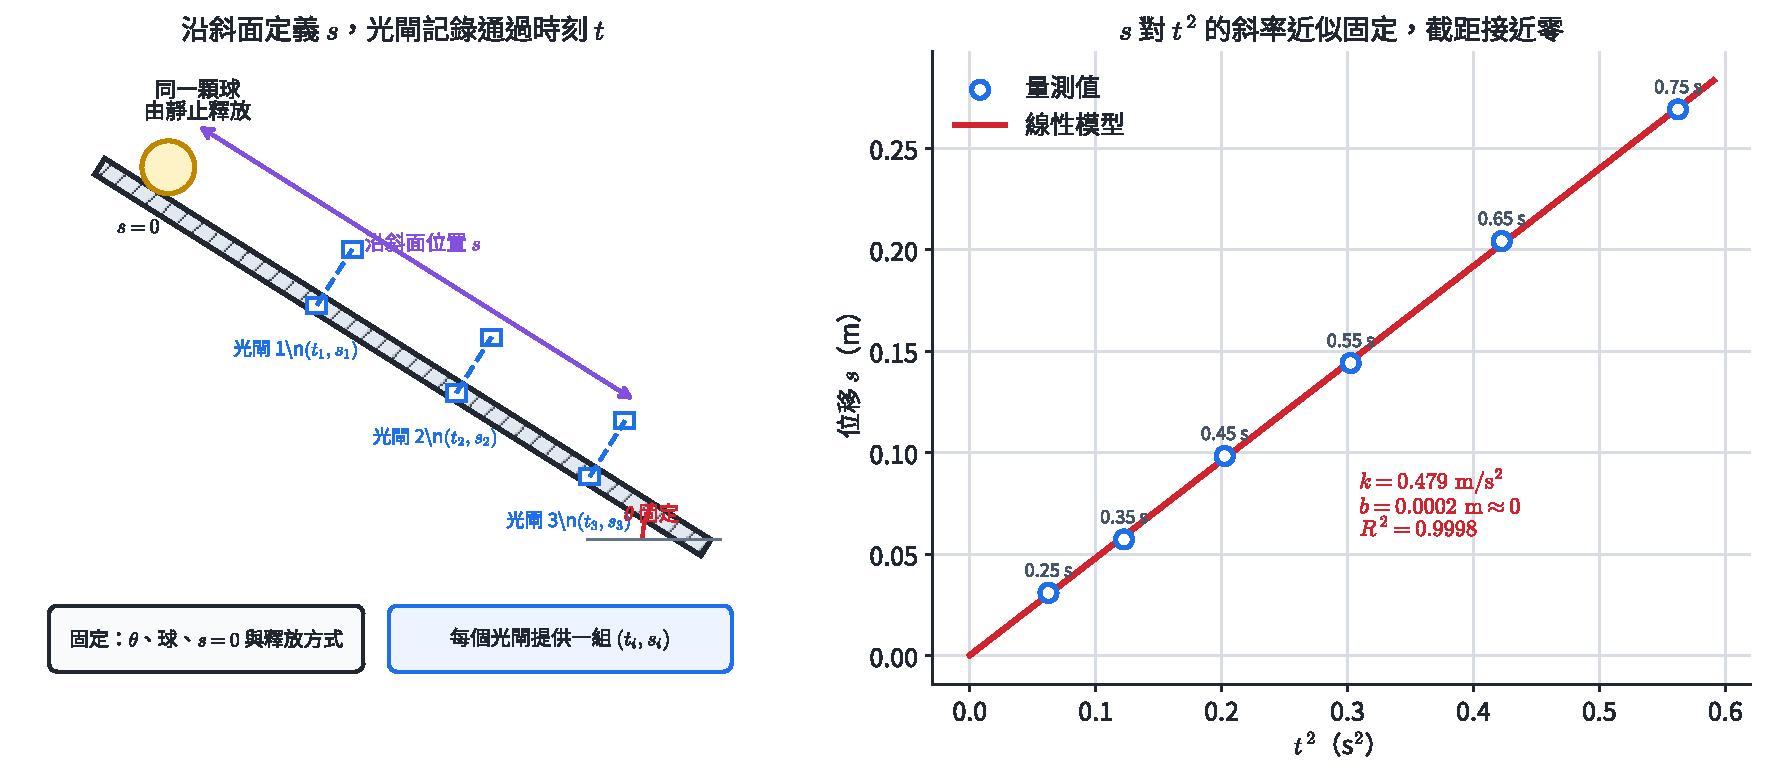
\includegraphics[keepaspectratio,alt={斜面實驗與資料模型}]{assets/必物-1-斜面實驗與資料模型.pdf}}
\caption{斜面實驗與資料模型}
\end{figure}

圖 2｜從釋放點定義沿斜面位置 \(s\)；已知位置 \(s_i\) 的光閘記錄通過時刻 \(t_i\)，每道光閘形成一組 \((t_i,s_i)\) 資料。

斜面角度、球、釋放位置與釋放方式固定。將多組資料的 \(s\) 對 \(t^2\) 作圖。資料接近直線表示

\[
s\approx kt^2,
\]

其中斜率 \(k\) 的單位為

\[
[k]=\frac{\mathrm m}{\mathrm{s^2}}.
\]

數學模型濃縮資料，也能產生新預測。例如量得 \(k\approx0.48\ \mathrm{m/s^2}\)，便可預測 \(t=0.80\ \mathrm s\) 時

\[
s\approx(0.48)(0.80)^2=0.307\ \mathrm m.
\]

模型的適用條件包含同一斜面角度、相同釋放方式與近似固定的阻力。改變斜角後，要重新量測 \(k\)。

\subsection{2.2 物理量與共同標準}\label{ux7269ux7406ux91cfux8207ux5171ux540cux6a19ux6e96}

物理量是可用數值與單位表示的物理性質。完整紀錄包含

\[
\text{物理量}=\text{數值}\times\text{單位}.
\]

「長度為 2.4」缺少比較基準；「長度為 \(2.4\ \mathrm m\)」才能與其他量測比較。共同單位使不同儀器、實驗室與國家的結果能互相複製。

國際單位制簡稱 SI，目前選定七個基本量與基本單位：

{\def\LTcaptype{none} % do not increment counter
\begin{longtable}[]{@{}llrl@{}}
\toprule\noalign{}
基本量 & 基本單位 & 代號 & 現行定義所連結的常數 \\
\midrule\noalign{}
\endhead
\bottomrule\noalign{}
\endlastfoot
時間 & 秒 & s & 銫-133 原子躍遷頻率 \\
長度 & 公尺 & m & 真空光速 \(c\) \\
質量 & 公斤 & kg & 普朗克常數 \(h\) \\
電流 & 安培 & A & 基本電荷 \(e\) \\
熱力學溫度 & 克耳文 & K & 波茲曼常數 \(k_{\mathrm B}\) \\
物量 & 莫耳 & mol & 亞佛加厥常數 \(N_{\mathrm A}\) \\
光強度 & 燭光 & cd & 特定頻率光的發光效能 \\
\end{longtable}
}

力學最常用長度、質量與時間，對應 m、kg、s，因此常稱 MKS 制。

秒以銫-133 原子特定躍遷的 \(9\,192\,631\,770\) 個週期定義。公尺利用固定的真空光速 \(299\,792\,458\ \mathrm{m/s}\) 定義。公斤自 2019 年起以固定普朗克常數

\[
h=6.626\,070\,15\times10^{-34}\ \mathrm{J\,s}
\]

的數值定義。以自然常數建立標準，可由具備相應儀器的實驗室重現，減少實體原器受灰塵、清洗或環境影響的問題。

\subsection{2.3 基本量與導出量}\label{ux57faux672cux91cfux8207ux5c0eux51faux91cf}

基本量由單位制選定；其他物理量依定義或定律由基本量組合，稱為導出量。導出單位必須沿公式中的乘除關係組合。

\begin{figure}
\centering
\pandocbounded{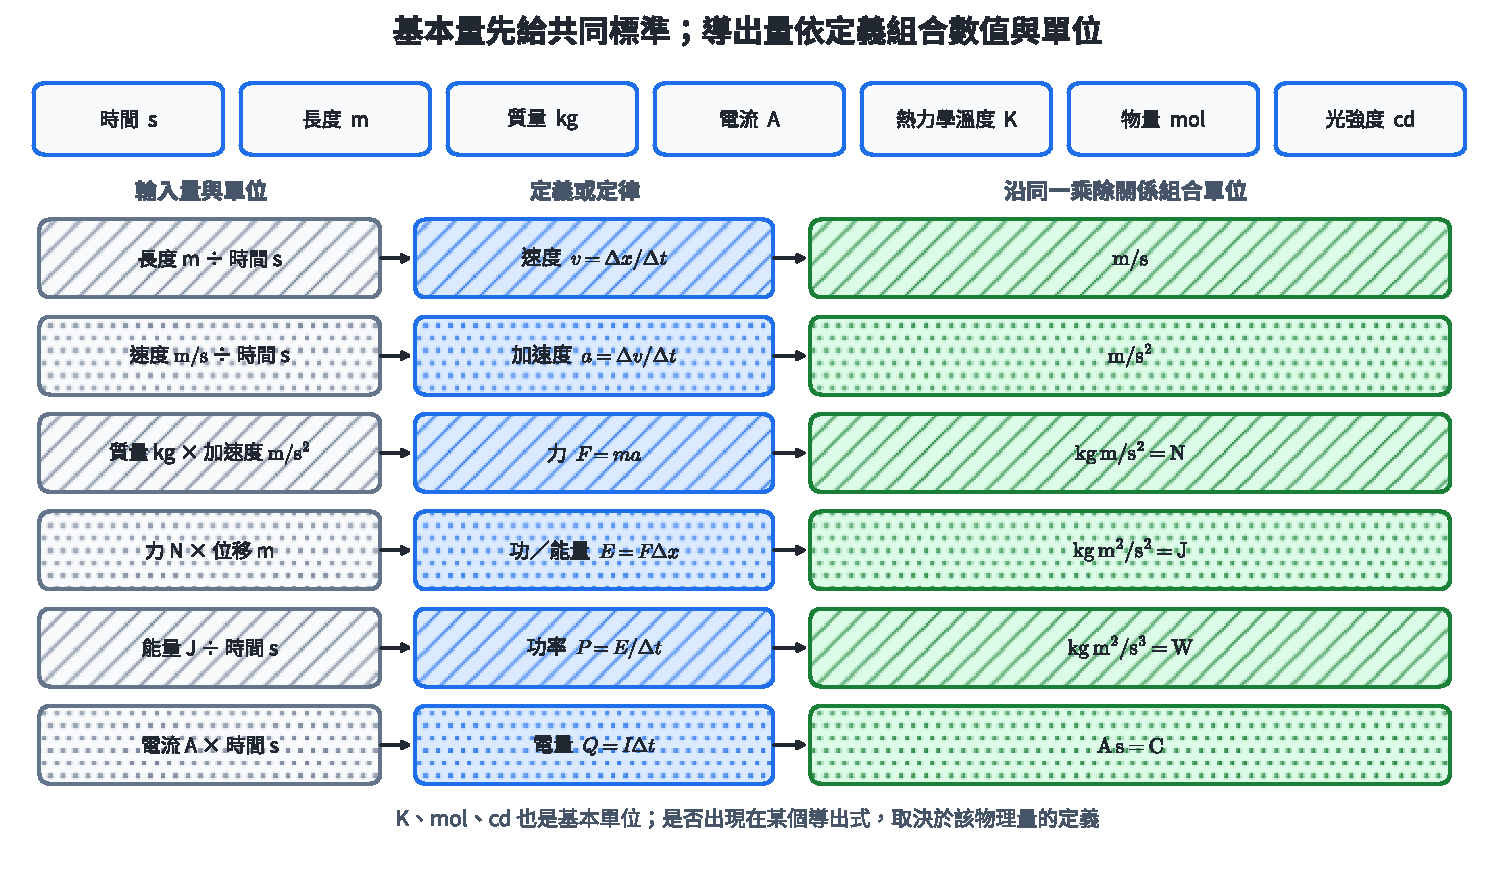
\includegraphics[keepaspectratio,alt={SI 基本量與導出量}]{assets/必物-1-SI基本量與導出量.pdf}}
\caption{SI 基本量與導出量}
\end{figure}

圖 3｜導出單位沿同一定義式的乘除關係組合；速度、加速度、力、能量、功率與電量的單位可由圖中逐列導出。

例如

\[
v=\frac{\Delta x}{\Delta t}
\quad\Rightarrow\quad
[v]=\frac{\mathrm m}{\mathrm s},
\]

\[
a=\frac{\Delta v}{\Delta t}
\quad\Rightarrow\quad
[a]=\frac{\mathrm m}{\mathrm{s^2}},
\]

\[
F=ma
\quad\Rightarrow\quad
[F]=\frac{\mathrm{kg\,m}}{\mathrm{s^2}}
\equiv \mathrm N.
\]

能量、功率與電量分別為

\[
[E]=\mathrm{N\,m}
=\frac{\mathrm{kg\,m^2}}{\mathrm{s^2}}
\equiv\mathrm J,
\]

\[
[P]=\frac{\mathrm J}{\mathrm s}
=\frac{\mathrm{kg\,m^2}}{\mathrm{s^3}}
\equiv\mathrm W,
\]

\[
[Q]=\mathrm{A\,s}
\equiv\mathrm C.
\]

牛頓、焦耳、瓦特與庫侖是導出單位的專名。判斷基本或導出時，要看物理量的定義來源，而非名稱是否常見。

單位一致性也是檢查公式的必要條件。若

\[
x=v_0t+\frac12at^2,
\]

右邊第一項單位為

\[
\frac{\mathrm m}{\mathrm s}\cdot\mathrm s=\mathrm m,
\]

第二項為

\[
\frac{\mathrm m}{\mathrm{s^2}}\cdot\mathrm{s^2}=\mathrm m,
\]

兩項才能相加並與左邊位移一致。單位一致只表示公式通過一項必要檢查；係數、正負號與適用條件仍要由推導或實驗決定。

\subsection{2.4 前綴詞、科學記號與換算}\label{ux524dux7db4ux8a5eux79d1ux5b78ux8a18ux865fux8207ux63dbux7b97}

尺度很大或很小時，可在 SI 單位前加前綴：

{\def\LTcaptype{none} % do not increment counter
\begin{longtable}[]{@{}lrrlrr@{}}
\toprule\noalign{}
前綴 & 代號 & 倍數 & 前綴 & 代號 & 倍數 \\
\midrule\noalign{}
\endhead
\bottomrule\noalign{}
\endlastfoot
拍 & P & \(10^{15}\) & 厘 & c & \(10^{-2}\) \\
兆 & T & \(10^{12}\) & 毫 & m & \(10^{-3}\) \\
吉 & G & \(10^9\) & 微 & \(\mu\) & \(10^{-6}\) \\
百萬 & M & \(10^6\) & 奈 & n & \(10^{-9}\) \\
千 & k & \(10^3\) & 皮 & p & \(10^{-12}\) \\
& & & 飛 & f & \(10^{-15}\) \\
& & & 阿 & a & \(10^{-18}\) \\
\end{longtable}
}

代號區分大小寫：\(\mathrm M=10^6\)，\(\mathrm m=10^{-3}\)。

\begin{figure}
\centering
\pandocbounded{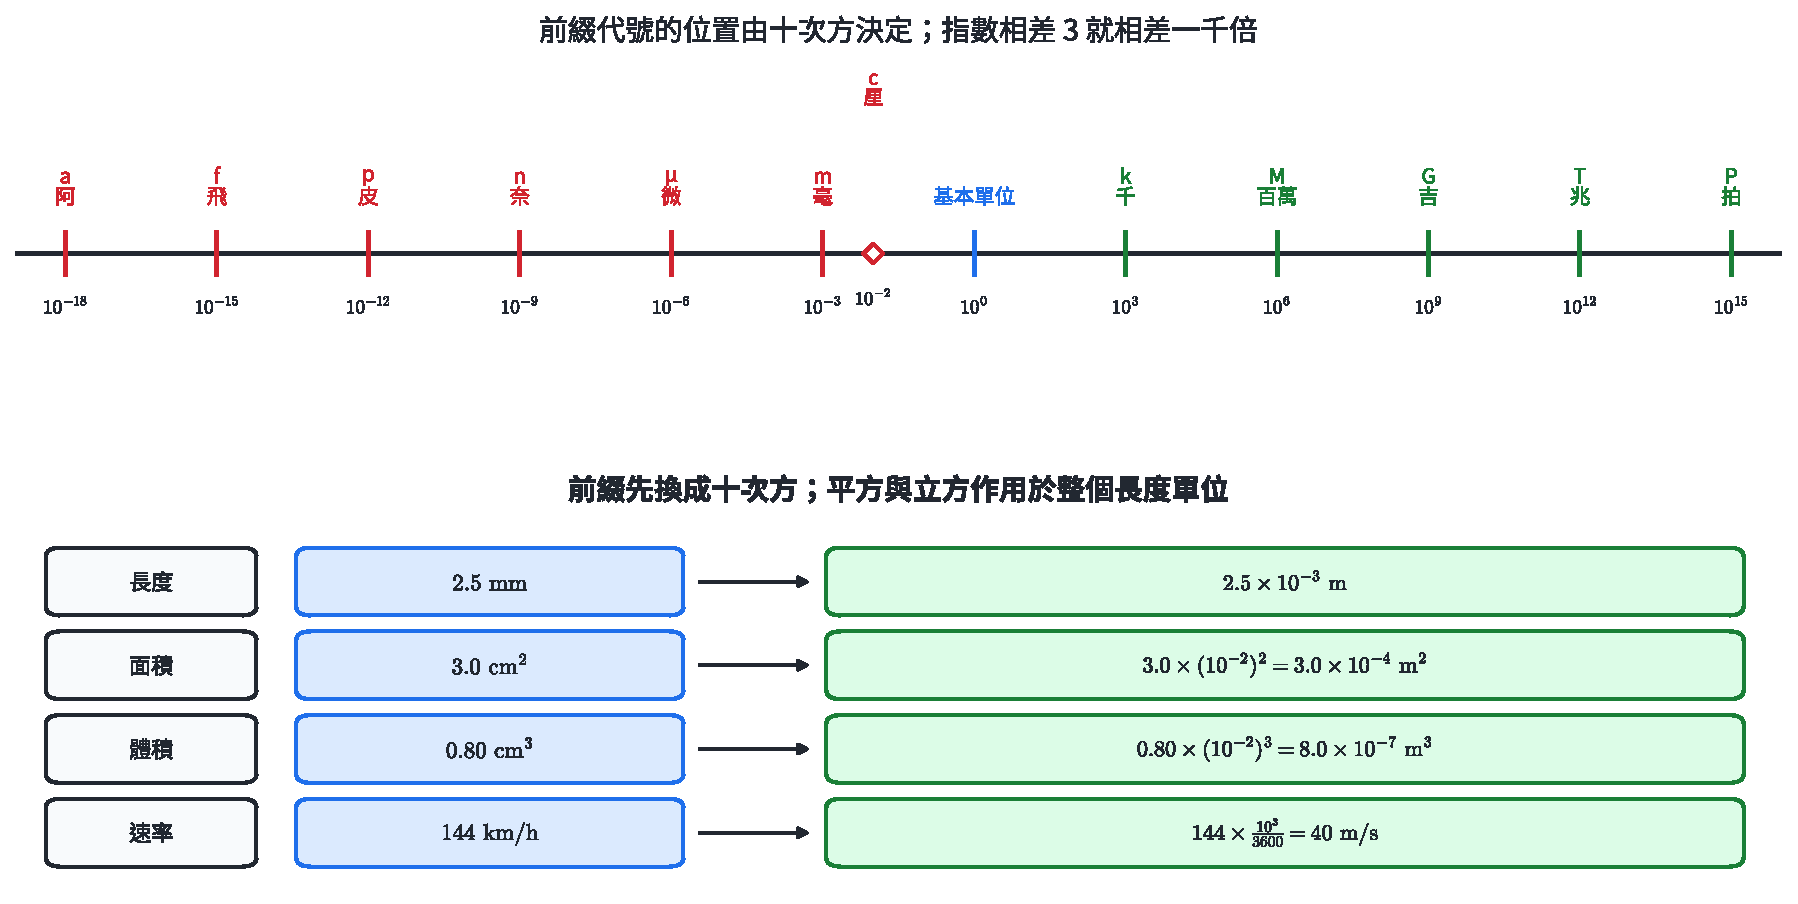
\includegraphics[keepaspectratio,alt={前綴詞與單位換算}]{assets/必物-1-前綴詞與單位換算.pdf}}
\caption{前綴詞與單位換算}
\end{figure}

圖 4｜前綴對應十次方；面積與體積換算時，單位內的前綴倍率也分別平方與立方。

換算時把前綴代成十次方，再讓平方或立方作用在整個單位上：

\[
1\ \mathrm{cm^2}
=(10^{-2}\ \mathrm m)^2
=10^{-4}\ \mathrm{m^2},
\]

\[
1\ \mathrm{cm^3}
=(10^{-2}\ \mathrm m)^3
=10^{-6}\ \mathrm{m^3}.
\]

複合單位的分子與分母都要換算。例如

\[
144\ \mathrm{km/h}
=144\frac{10^3\ \mathrm m}{3600\ \mathrm s}
=40\ \mathrm{m/s}.
\]

科學記號寫成

\[
x=a\times10^n,\qquad 1\leq a<10.
\]

它把有效的數值部分與尺度分開。例如 \(0.000\,0025\ \mathrm m=2.5\times10^{-6}\ \mathrm m=2.5\ \mu\mathrm m\)。

\subsection{2.5 數量級與估算}\label{ux6578ux91cfux7d1aux8207ux4f30ux7b97}

數量級以最接近的十次方粗略描述數值大小。若

\[
x=a\times10^n,\qquad 1\leq a<10,
\]

則以 \(\sqrt{10}\approx3.16\) 為分界：

\[
\begin{cases}
a<\sqrt{10}, & x\text{ 的數量級為 }10^n,\\
a\geq\sqrt{10}, & x\text{ 的數量級為 }10^{n+1}.
\end{cases}
\]

例如 \(2.4\times10^5\) 的數量級為 \(10^5\)；\(6.0\times10^5\) 的數量級為 \(10^6\)。數量級適合快速估算、比較尺度及檢查計算結果。

\begin{figure}
\centering
\pandocbounded{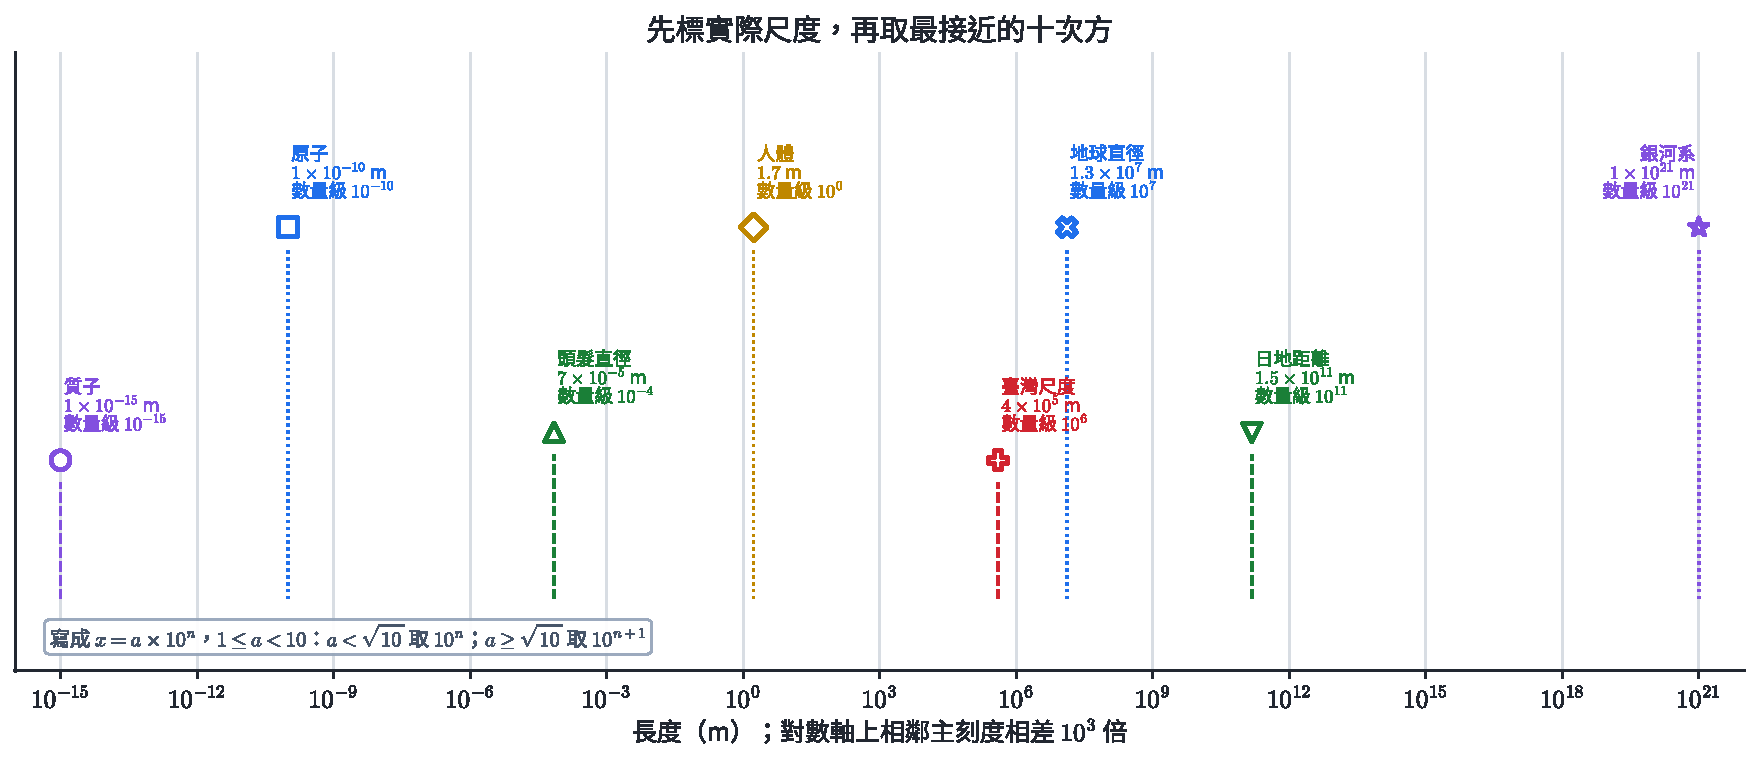
\includegraphics[keepaspectratio,alt={長度尺度與數量級}]{assets/必物-1-長度尺度與數量級.pdf}}
\caption{長度尺度與數量級}
\end{figure}

圖 5｜標記實際尺度後，以係數 \(a\) 和 \(\sqrt{10}\) 比較，才能選出最接近的十次方。

對數軸上的等距代表相同倍率。原子約 \(10^{-10}\ \mathrm m\)，人體約 \(10^0\ \mathrm m\)，兩者相差約十個數量級；日地距離約 \(1.5\times10^{11}\ \mathrm m\)。

\subsubsection{示範 4　由斜面資料檢查比例模型}\label{ux793aux7bc4-4-ux7531ux659cux9762ux8cc7ux6599ux6aa2ux67e5ux6bd4ux4f8bux6a21ux578b}

量得：

{\def\LTcaptype{none} % do not increment counter
\begin{longtable}[]{@{}rrrrrrr@{}}
\toprule\noalign{}
\(t\)（s） & 0.25 & 0.35 & 0.45 & 0.55 & 0.65 & 0.75 \\
\midrule\noalign{}
\endhead
\bottomrule\noalign{}
\endlastfoot
\(s\)（m） & 0.0310 & 0.0573 & 0.0984 & 0.1442 & 0.2043 & 0.2692 \\
\end{longtable}
}

計算 \(s/t^2\)：

\[
0.496,\ 0.468,\ 0.486,\ 0.477,\ 0.484,\ 0.479
\quad(\mathrm{m/s^2}).
\]

各值集中在 \(0.48\ \mathrm{m/s^2}\) 附近，且圖上的 \(s-t^2\) 資料接近直線，因此資料支持

\[
s\approx(0.48\ \mathrm{m/s^2})t^2.
\]

比值的離散顯示實際量測有起伏；模型係數寫成近似值。

\subsubsection{示範 5　設計公平比較}\label{ux793aux7bc4-5-ux8a2dux8a08ux516cux5e73ux6bd4ux8f03}

問題：斜面角度增加是否會縮短球移動 \(0.80\ \mathrm m\) 所需時間？

\begin{enumerate}
\def\labelenumi{\arabic{enumi}.}
\tightlist
\item
  自變量：斜面角度，例如 \(5^\circ,10^\circ,15^\circ\)。
\item
  應變量：由靜止移動 \(0.80\ \mathrm m\) 的時間。
\item
  控制變因：同一顆球、同一路面、同一距離、同一釋放器與計時器。
\item
  操作定義：球脫離釋放器時開始計時，通過終點光閘時停止。
\item
  重複：每個角度至少量多次，報告原始值與代表值。
\item
  資料圖：橫軸角度、縱軸時間，並標示各角度的量測離散。
\end{enumerate}

這個設計把角度的影響與球、路面及釋放方式分開。

\subsubsection{示範 6　由定義推導導出單位}\label{ux793aux7bc4-6-ux7531ux5b9aux7fa9ux63a8ux5c0eux5c0eux51faux55aeux4f4d}

壓力定義為單位面積所受的力：

\[
p=\frac FA.
\]

所以

\[
[p]=\frac{\mathrm N}{\mathrm{m^2}}
=\frac{\mathrm{kg\,m/s^2}}{\mathrm{m^2}}
=\frac{\mathrm{kg}}{\mathrm{m\,s^2}}
\equiv\mathrm{Pa}.
\]

比熱定義為使單位質量升高單位溫度所需的熱量：

\[
c=\frac{Q}{m\Delta T}.
\]

其 SI 單位為

\[
[c]=\frac{\mathrm J}{\mathrm{kg\,K}}
=\frac{\mathrm{m^2}}{\mathrm{s^2\,K}}.
\]

兩種寫法等價，後者把焦耳拆成基本單位。

\subsubsection{示範 7　用單位檢查公式}\label{ux793aux7bc4-7-ux7528ux55aeux4f4dux6aa2ux67e5ux516cux5f0f}

有人寫出行進距離

\[
d=vt+\frac12at.
\]

第一項 \(vt\) 的單位是 m。第二項 \(at\) 的單位為

\[
\frac{\mathrm m}{\mathrm{s^2}}\cdot\mathrm s
=\frac{\mathrm m}{\mathrm s},
\]

兩項單位不同，無法相加。若第二項為 \(\frac12at^2\)，單位才是 m。這項檢查能指出式子少了一個時間因子。

\subsubsection{示範 8　前綴與立方單位}\label{ux793aux7bc4-8-ux524dux7db4ux8207ux7acbux65b9ux55aeux4f4d}

體積 \(0.80\ \mathrm{cm^3}\) 換成 \(\mathrm{m^3}\)：

\[
0.80\ \mathrm{cm^3}
=0.80(10^{-2}\ \mathrm m)^3
=0.80\times10^{-6}\ \mathrm{m^3}
=8.0\times10^{-7}\ \mathrm{m^3}.
\]

無線電頻率 \(103.3\ \mathrm{MHz}\)：

\[
103.3\ \mathrm{MHz}
=103.3\times10^6\ \mathrm{Hz}
=1.033\times10^8\ \mathrm{Hz}.
\]

\subsubsection{示範 9　數量級估算}\label{ux793aux7bc4-9-ux6578ux91cfux7d1aux4f30ux7b97}

日地平均距離約 \(1.5\times10^{11}\ \mathrm m\)，光速約 \(3.0\times10^8\ \mathrm{m/s}\)：

\[
t=\frac dc
\approx\frac{1.5\times10^{11}}{3.0\times10^8}
=5.0\times10^2\ \mathrm s.
\]

因係數 \(5.0>\sqrt{10}\)，此時間的數量級為 \(10^3\ \mathrm s\)。精確到常用尺度約為 \(500\ \mathrm s\)，即約 \(8.3\) 分鐘。

\subsection{2.6 節內練習}\label{ux7bc0ux5167ux7df4ux7fd2-1}

\begin{enumerate}
\def\labelenumi{\arabic{enumi}.}
\tightlist
\item
  研究「電池溫度是否影響手電筒持續點亮時間」。分別寫出自變量、應變量、三個控制變因與一項操作定義。
\item
  同一斜面量得 \((t,s)=(0.20,0.020),(0.40,0.081),(0.60,0.181),(0.80,0.319)\)，單位分別為 s 與 m。計算各筆 \(s/t^2\)，判斷 \(s\propto t^2\) 是否合理。
\item
  從下列物理量選出 SI 基本量：能量、電流、時間、速度、物量、壓力、光強度。
\item
  由定義求 SI 基本單位表示：(a) 密度 \(\rho=m/V\)；(b) 動量 \(p=mv\)；(c) 壓力 \(p=F/A\)。
\item
  完成換算：(a) \(72\ \mathrm{km/h}\) 換成 m/s；(b) \(2.5\ \mathrm{mm^2}\) 換成 \(\mathrm{m^2}\)；(c) \(3.0\ \mathrm{GB}\) 換成 B，取 \(1\ \mathrm G=10^9\)。
\item
  判斷數量級：(a) \(2.8\times10^{-7}\ \mathrm m\)；(b) \(7.0\times10^{-7}\ \mathrm m\)；(c) 比較 \(10^{-10}\ \mathrm m\) 原子與 \(10^{-15}\ \mathrm m\) 質子的尺度倍率。
\end{enumerate}

\subsubsection{節內練習解析}\label{ux7bc0ux5167ux7df4ux7fd2ux89e3ux6790-1}

\begin{enumerate}
\def\labelenumi{\arabic{enumi}.}
\tightlist
\item
  自變量為電池溫度；應變量為達到事先訂定亮度下限前的時間。可控制電池型號與初始電量、燈泡、環境、電路及亮度判準；操作定義要說明溫度如何穩定及點亮終點如何判定。
\item
  \(s/t^2=0.500,0.506,0.503,0.498\ \mathrm{m/s^2}\)，集中在 \(0.50\ \mathrm{m/s^2}\) 附近，比例模型合理。
\item
  電流、時間、物量、光強度為基本量；其餘為導出量。
\item
  \begin{enumerate}
  \def\labelenumii{(\alph{enumii})}
  \tightlist
  \item
    \(\mathrm{kg/m^3}\)；(b) \(\mathrm{kg\,m/s}\)；(c) \(\mathrm{kg/(m\,s^2)}\)。
  \end{enumerate}
\item
  \begin{enumerate}
  \def\labelenumii{(\alph{enumii})}
  \tightlist
  \item
    \(72/3.6=20\ \mathrm{m/s}\)；(b) \(2.5(10^{-3})^2=2.5\times10^{-6}\ \mathrm{m^2}\)；(c) \(3.0\times10^9\ \mathrm B\)。
  \end{enumerate}
\item
  \begin{enumerate}
  \def\labelenumii{(\alph{enumii})}
  \tightlist
  \item
    係數 \(2.8<3.16\)，數量級 \(10^{-7}\ \mathrm m\)；(b) 係數 \(7.0>3.16\)，數量級 \(10^{-6}\ \mathrm m\)；(c) 相差 \(10^{-10}/10^{-15}=10^5\) 倍。
  \end{enumerate}
\end{enumerate}

\section{3　物理學簡介}\label{ux7269ux7406ux5b78ux7c21ux4ecb}

\subsection{3.1 探究方向、領域與模型條件}\label{ux63a2ux7a76ux65b9ux5411ux9818ux57dfux8207ux6a21ux578bux689dux4ef6}

物理學研究物質結構、運動、能量、交互作用與宇宙演化，尺度可從原子內部延伸到天體。古典物理常分成四個主要領域：

\begin{itemize}
\tightlist
\item
  力學：物體運動、平衡與造成狀態改變的作用。
\item
  熱學：溫度、內能、熱傳與能量轉換。
\item
  電磁學：電荷、電流、電場、磁場及電磁波。
\item
  光學：光的反射、折射、干涉、繞射與成像。
\end{itemize}

近代物理主要包含量子理論與相對論。量子模型處理原子、電子、光子與微觀尺度的離散及機率現象；相對論處理速度接近光速或重力很強的系統。

\begin{figure}
\centering
\pandocbounded{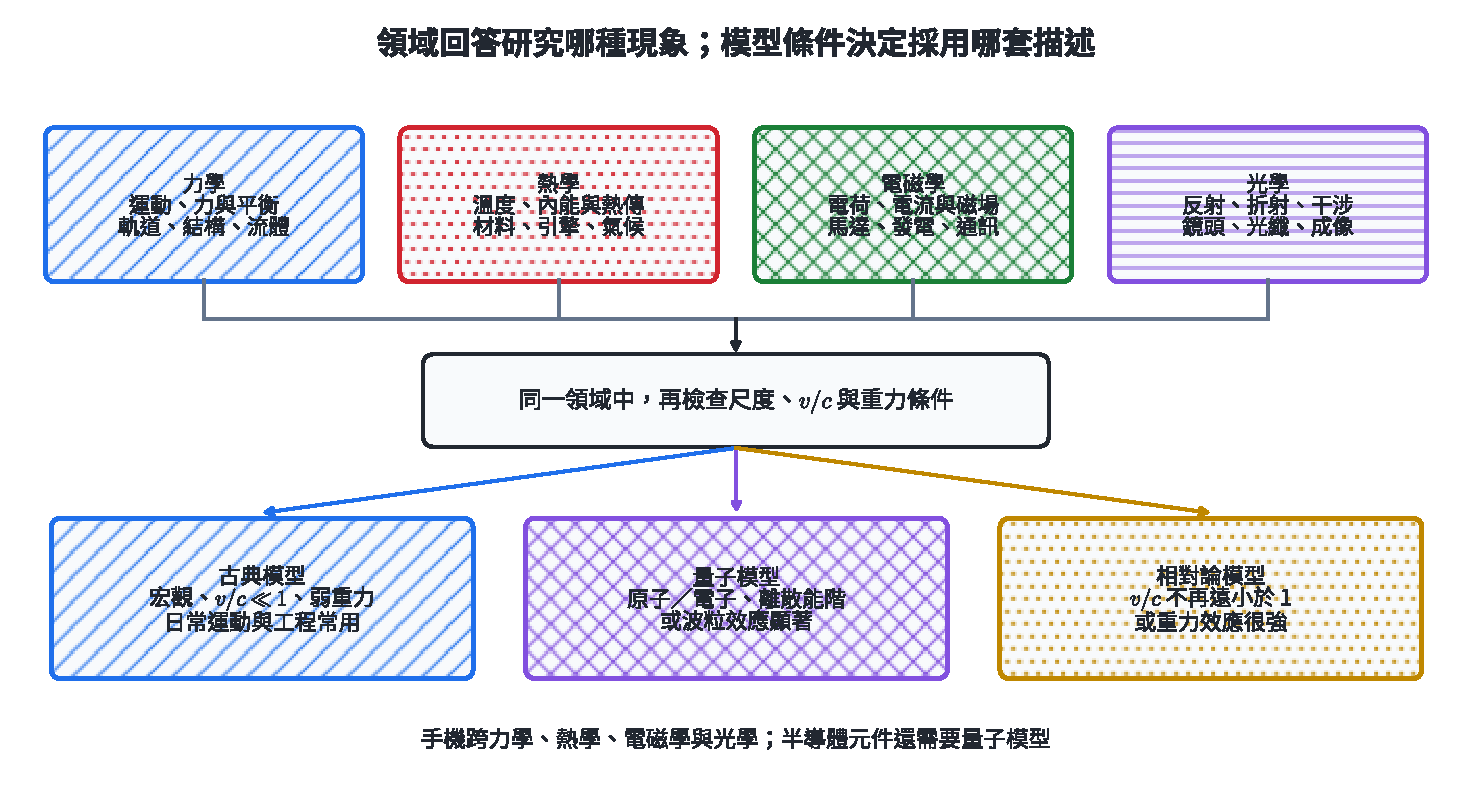
\includegraphics[keepaspectratio,alt={物理領域與模型條件}]{assets/必物-1-物理領域與模型條件.pdf}}
\caption{物理領域與模型條件}
\end{figure}

圖 6｜領域依研究現象分類；在同一領域內，還要依尺度、\(v/c\) 與重力條件選擇古典、量子或相對論模型。

領域是依研究問題分類，模型則依條件選擇。同一裝置可跨領域：手機包含力學加速度感測、電磁通訊、熱管理、光學鏡頭及量子半導體。日常低速、宏觀、弱重力條件下，古典模型通常已有足夠精度；尺度、速度或重力條件改變時，再選用近代模型。

模型的適用條件是模型的一部分。使用一條定律時，要同時說明對象、尺度、速度、交互作用及忽略因素。這能避免把「某條件下的準確近似」誤當成所有尺度都相同。

\subsection{3.2 物理學的發展：證據、數學與統一}\label{ux7269ux7406ux5b78ux7684ux767cux5c55ux8b49ux64daux6578ux5b78ux8207ux7d71ux4e00}

紀元前六世紀的泰勒斯嘗試以自然界本身的原因說明現象，代表古希臘自然哲學以概念與論證理解自然的轉變。近代物理學的形成，則進一步把精確觀測、控制實驗與數學模型結合。

哥白尼以可計算的日心模型重新組織天文現象。克卜勒依第谷的大量觀測資料，把正圓軌道修正為橢圓並歸納行星運動定律。伽利略以斜面實驗研究運動，顯示距離與時間平方的數學關係。笛卡兒以廣度、位置與運動描述物質，並把現象對應為可由幾何與運動分析的機制；這項思路促進了可數學化機械觀的形成。牛頓再以運動定律與萬有引力，把地表落體與月球、行星運動放進同一力學架構。

十九世紀的發展呈現另一條統一鏈：

\begin{enumerate}
\def\labelenumi{\arabic{enumi}.}
\tightlist
\item
  厄斯特觀察到通電導線使磁針偏轉，建立電與磁的實驗連結。
\item
  法拉第發現隨時間變動的磁場能在線圈中產生電流。
\item
  馬克士威把電磁實驗寫成方程，預測電磁波，並指出光是電磁波。
\item
  焦耳與麥爾由實驗建立功與熱的轉換關係，使能量成為跨力學與熱學的共同概念。
\end{enumerate}

二十世紀初，古典理論無法完整解釋黑體輻射，也需處理光速測量與運動的關係。普朗克以能量量子化解釋黑體頻譜；愛因斯坦提出光子模型與相對論，開啟近代物理。

\begin{figure}
\centering
\pandocbounded{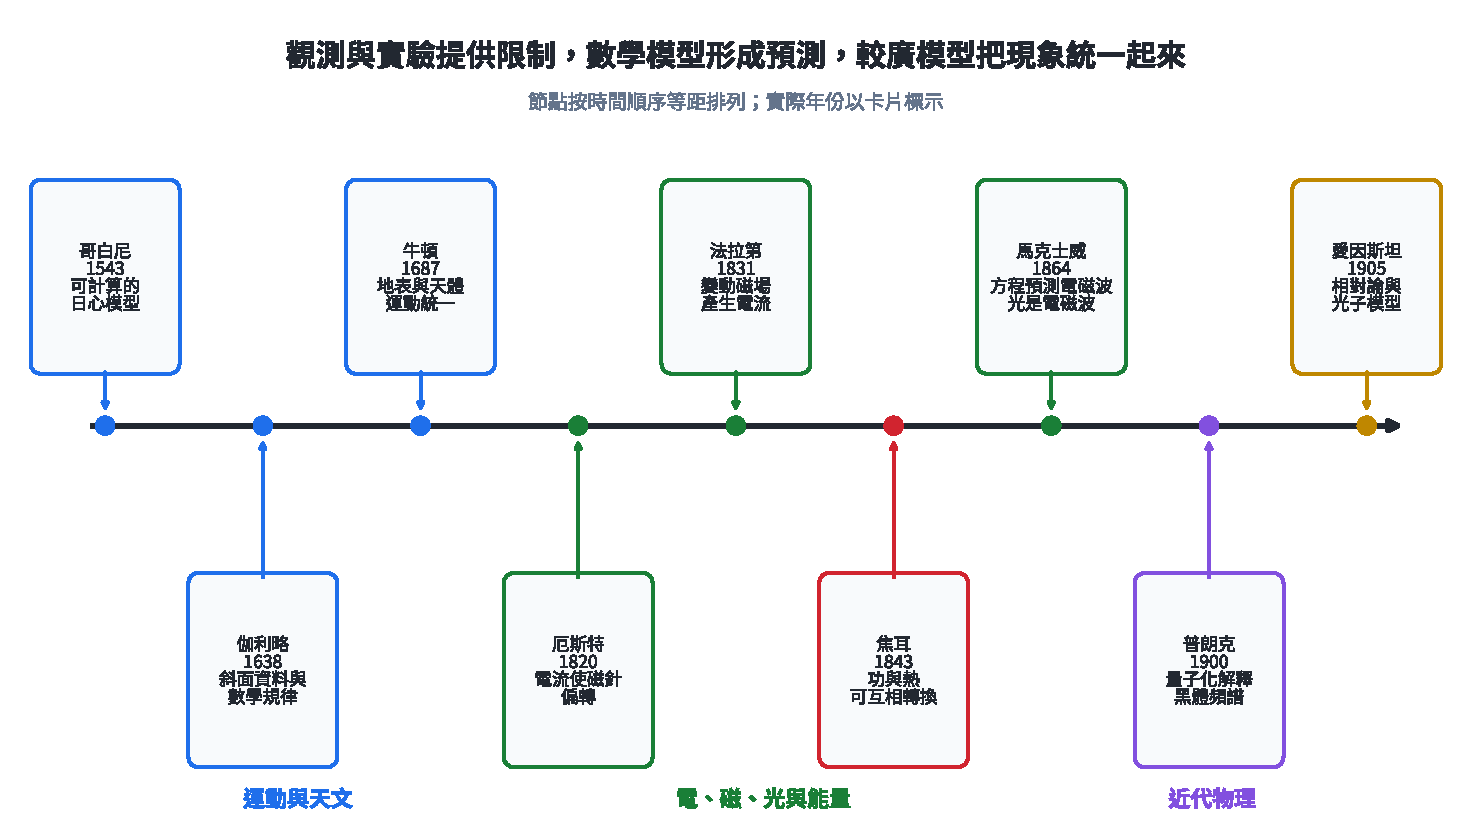
\includegraphics[keepaspectratio,alt={物理史的證據、模型與統一}]{assets/必物-1-物理史的證據模型與統一.pdf}}
\caption{物理史的證據、模型與統一}
\end{figure}

圖 7｜節點依年份順序等距排列，等距不代表實際時距；卡片列出證據、模型、預測或統一現象的具體進展。

物理史的主線不只是人名與年代，而是三種進展：

\begin{itemize}
\tightlist
\item
  新儀器或新資料限制舊解釋。
\item
  數學模型把多筆資料壓縮成可計算規律。
\item
  更廣模型把原先分開的現象放進同一原理，並做出新預測。
\end{itemize}

\subsection{3.3 跨學科合作}\label{ux8de8ux5b78ux79d1ux5408ux4f5c}

現代科技系統常把多個學科接成完整證據鏈。電腦斷層使用 X 光與物質交互作用、穩定光源與偵測器、多角度資料、數學重建與臨床判讀。每一環都需共同單位、校正標準與可重複程序。

\begin{figure}
\centering
\pandocbounded{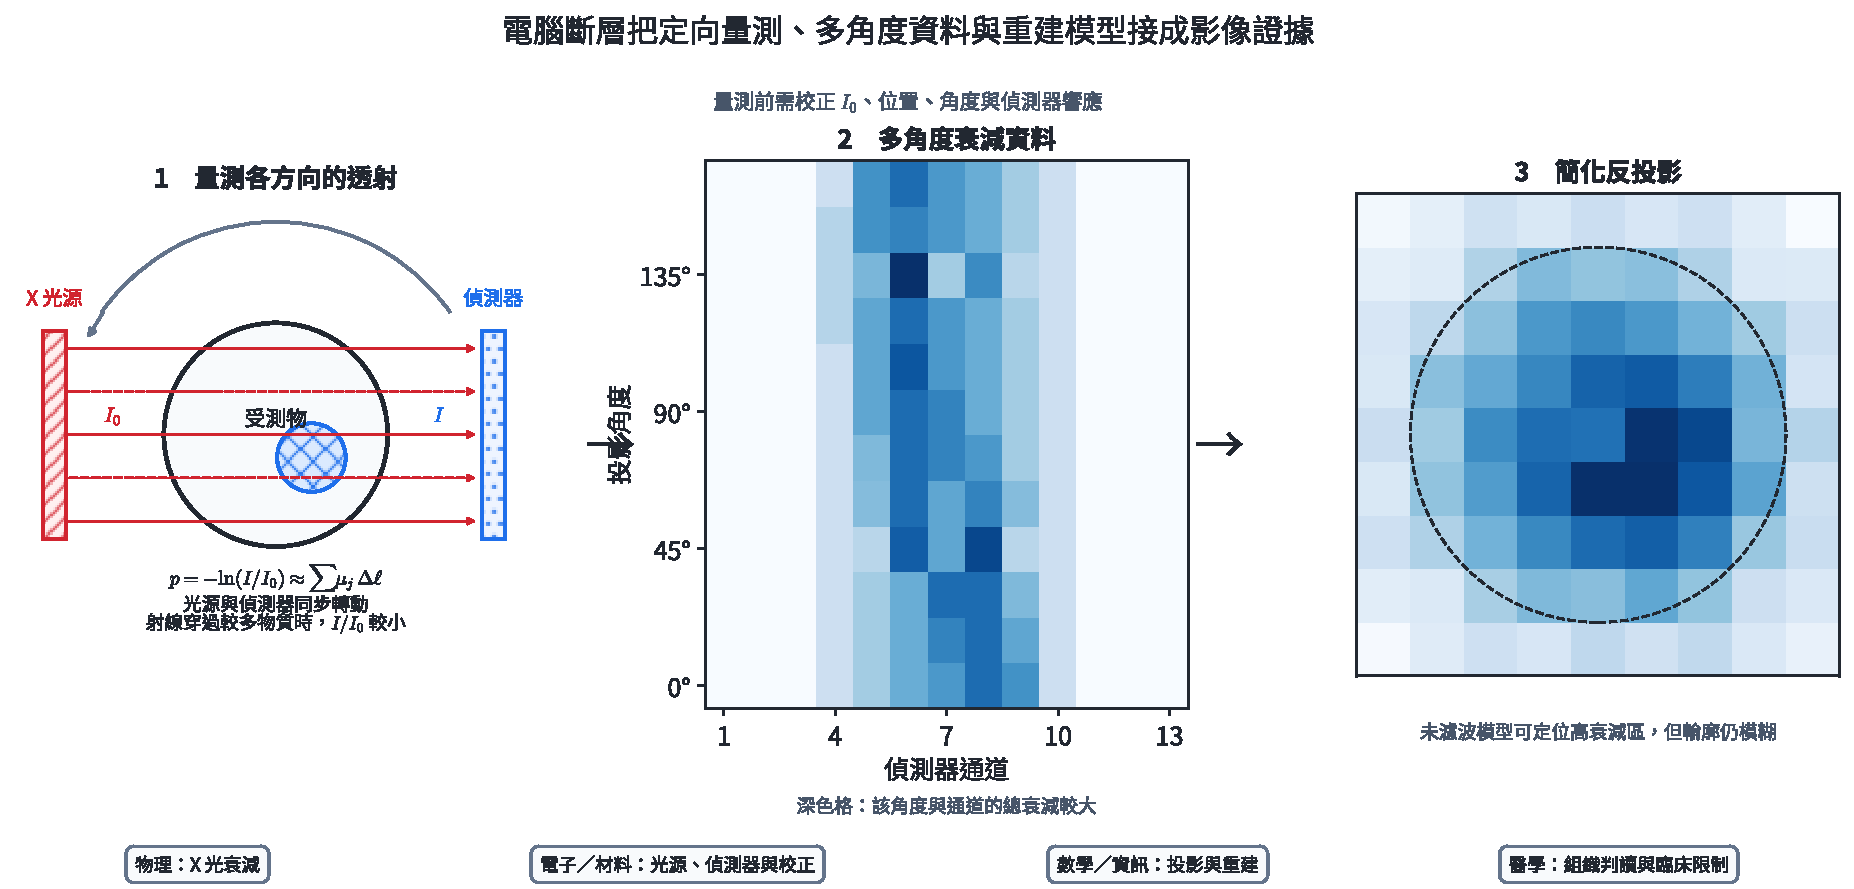
\includegraphics[keepaspectratio,alt={跨領域電腦斷層系統}]{assets/必物-1-跨領域電腦斷層系統.pdf}}
\caption{跨領域電腦斷層系統}
\end{figure}

圖 8｜左圖的平行 X 光從光源射向偵測器；中圖每一格由對應角度與通道的投影和計算，右圖將這些數值做簡化反投影。

圖中以 \(9\times9\) 衰減系數模型和 \(12\) 個投影角度示範。中圖數值由左圖模型的定向投影計算；右圖是未濾波反投影，因此可定位高衰減區，輪廓仍較模糊。實際電腦斷層使用更多射線與角度，並加入完整校正與濾波重建。

圖中：

\begin{enumerate}
\def\labelenumi{\arabic{enumi}.}
\tightlist
\item
  物理提供 X 光傳播與衰減模型。
\item
  電子與材料工程提供光源、偵測器及校正。
\item
  數學與資訊把不同角度的資料重建成切面影像。
\item
  醫學判讀影像，並界定劑量、適用情境與臨床限制。
\end{enumerate}

智慧型手機、磁振造影、超音波、積體電路與發光二極體也具有相似結構。跨學科合作的關鍵是把各專業的量測、模型與判準明確接合，而非只把不同專家列在同一名單。

\subsubsection{示範 10　由問題選領域}\label{ux793aux7bc4-10-ux7531ux554fux984cux9078ux9818ux57df}

\begin{enumerate}
\def\labelenumi{\arabic{enumi}.}
\tightlist
\item
  橋梁受風後的振動頻率：以力學描述結構運動。
\item
  保溫瓶散熱速率：以熱學描述能量傳遞。
\item
  發電機線圈中的感應電流：以電磁學描述變動磁場與電流。
\item
  相機鏡頭的成像與色差：以光學描述折射及成像。
\item
  原子只吸收特定波長：以量子能階模型描述。
\end{enumerate}

實際問題常有第二領域，例如相機也要處理電子感測與熱雜訊；先找主導觀測量，再加入必要模型。

\subsubsection{示範 11　重建運動模型的發展鏈}\label{ux793aux7bc4-11-ux91cdux5efaux904bux52d5ux6a21ux578bux7684ux767cux5c55ux93c8}

給定四項資料：

\begin{itemize}
\tightlist
\item
  伽利略以斜面量測得到運動的數學規律。
\item
  哥白尼提出較簡潔的日心架構。
\item
  牛頓用萬有引力統一地表與天體運動。
\item
  克卜勒依觀測把行星軌道改為橢圓。
\end{itemize}

合理的推理順序為：

\[
\text{哥白尼模型}
\rightarrow
\text{克卜勒以資料修正軌道}
\rightarrow
\text{伽利略建立地表運動規律}
\rightarrow
\text{牛頓完成統一模型}.
\]

其中「模型更簡潔」「符合觀測資料」「由實驗建立數學規律」「統一兩類現象」分別代表不同科學貢獻。

\subsubsection{示範 12　電磁學中的實驗與預測}\label{ux793aux7bc4-12-ux96fbux78c1ux5b78ux4e2dux7684ux5be6ux9a57ux8207ux9810ux6e2c}

厄斯特的磁針偏轉是直接觀察；法拉第的線圈實驗顯示變動磁場能產生電流；馬克士威把這些關係寫成方程並預測電磁波。

若題目問「首先由實驗發現電磁感應」，對應法拉第。若問「由方程預測電磁波並把光納入電磁現象」，對應馬克士威。判斷依據是動詞與證據型態，而非只背名字。

\subsubsection{示範 13　依條件選模型}\label{ux793aux7bc4-13-ux4f9dux689dux4ef6ux9078ux6a21ux578b}

\begin{enumerate}
\def\labelenumi{\arabic{enumi}.}
\tightlist
\item
  棒球速率 \(30\ \mathrm{m/s}\)、尺度約 \(0.1\ \mathrm m\)：\(v/c\approx10^{-7}\)，古典力學適用。
\item
  電子位於原子內，尺度約 \(10^{-10}\ \mathrm m\)：使用量子模型。
\item
  太空船速率 \(0.80c\)：時間與長度關係需相對論修正。
\end{enumerate}

同一物理量「位置」在三種情況都可測量，但描述其演化的模型不同。

\subsubsection{示範 14　拆解電腦斷層的證據鏈}\label{ux793aux7bc4-14-ux62c6ux89e3ux96fbux8166ux65b7ux5c64ux7684ux8b49ux64daux93c8}

若重建影像出現一處亮區，完整推理包含：

\begin{enumerate}
\def\labelenumi{\arabic{enumi}.}
\tightlist
\item
  原始偵測器讀值是否通過校正。
\item
  多角度資料是否在相同位置與單位系統下合併。
\item
  重建演算法是否經已知樣本測試。
\item
  亮區在重複掃描或其他成像方法中是否穩定。
\item
  臨床上哪些組織或材料可能產生相似訊號。
\end{enumerate}

「亮區」是影像資料；「某種組織異常」是專業解釋。兩者之間要有校正、模型與交叉證據。

\subsection{3.4 節內練習}\label{ux7bc0ux5167ux7df4ux7fd2-2}

\begin{enumerate}
\def\labelenumi{\arabic{enumi}.}
\tightlist
\item
  分類主要領域：輪胎煞車距離、鍋中水的升溫、馬達轉動、光纖傳訊、原子光譜。
\item
  分別選擇主要模型：低速列車運動、電子晶體繞射、靠近強重力天體的時鐘、透鏡成像。
\item
  將哥白尼、伽利略、笛卡兒、牛頓、厄斯特、法拉第、馬克士威、普朗克依時間先後排列。
\item
  配對貢獻：焦耳、馬克士威、普朗克、愛因斯坦，分別對應功熱轉換、電磁波預測、能量量子化、相對論。
\item
  磁振造影需要磁場、射頻訊號、電子偵測、影像重建與醫學判讀。指出至少三個相關領域與各自工作。
\item
  一個模型能解釋既有資料，另一個模型除了解釋資料還成功預測新現象。哪一項證據使第二個模型更強？說明理由。
\end{enumerate}

\subsubsection{節內練習解析}\label{ux7bc0ux5167ux7df4ux7fd2ux89e3ux6790-2}

\begin{enumerate}
\def\labelenumi{\arabic{enumi}.}
\tightlist
\item
  依序為力學、熱學、電磁學、光學與電磁學、量子物理。
\item
  低速列車用古典力學；電子繞射用量子物質波；強重力時鐘用廣義相對論；透鏡成像用幾何光學。
\item
  哥白尼、伽利略、笛卡兒、牛頓、厄斯特、法拉第、馬克士威、普朗克。
\item
  焦耳---功熱轉換；馬克士威---電磁波與光的統一；普朗克---量子化；愛因斯坦---相對論。
\item
  物理處理磁場與訊號；電子／材料處理線圈與偵測器；數學／資訊重建影像；醫學判讀組織與限制，任三項。
\item
  成功預測尚未用來建立模型的新現象，使模型接受獨立檢驗，降低只為既有資料事後調整的可能。
\end{enumerate}

\section{4　章末分層題}\label{ux7ae0ux672bux5206ux5c64ux984c}

第 1--4 題處理科學態度與實驗，第 5--8 題處理 SI、換算與數量級，第 9--12 題處理物理領域與發展，第 13--16 題整合兩個以上主節。

\subsection{基礎與模型題}\label{ux57faux790eux8207ux6a21ux578bux984c}

\begin{enumerate}
\def\labelenumi{\arabic{enumi}.}
\item
  實驗記錄寫道：「加熱 5 分鐘後，金屬線長度由 \(1.0000\ \mathrm m\) 變成 \(1.0012\ \mathrm m\)，顯示粒子平均距離變大。」指出其中的直接觀察與模型解釋。
\item
  將「磁鐵愈強，吸起的迴紋針愈多」改寫成包含自變量、應變量、控制變因與操作定義的可檢驗假設。
\item
  一組量測值為 \(9.8,9.7,9.9,14.2,9.8\ \mathrm{m/s^2}\)。說明處理 \(14.2\) 這筆資料的科學程序。
\item
  研究斜面角度對小車通過固定距離時間的影響。寫出自變量、應變量、三個控制變因，並說明為何每個角度要重複量測。
\item
  從下列選出 SI 基本量：質量、力、電流、能量、熱力學溫度、速度、物量。
\item
  已知功率 \(P=E/t\)，能量 \(E=Fs\)，力 \(F=ma\)。把功率單位拆成 kg、m、s。
\item
  完成換算：

  \begin{enumerate}
  \def\labelenumii{(\arabic{enumii})}
  \tightlist
  \item
    \(90\ \mathrm{km/h}\) 換成 m/s。\\
  \item
    \(4.0\ \mathrm{cm^2}\) 換成 \(\mathrm{m^2}\)。\\
  \item
    \(650\ \mathrm{nm}\) 換成 m。
  \end{enumerate}
\item
  判斷下列數值的數量級：

  \begin{enumerate}
  \def\labelenumii{(\arabic{enumii})}
  \tightlist
  \item
    \(2.0\times10^6\)。\\
  \item
    \(5.0\times10^6\)。\\
  \item
    太陽質量 \(2.0\times10^{30}\ \mathrm{kg}\) 與地球質量 \(6.0\times10^{24}\ \mathrm{kg}\) 的比值。
  \end{enumerate}
\item
  指出主要領域：汽車轉彎、冷氣機搬運熱量、變壓器、望遠鏡成像、電子能階。
\item
  將下列里程碑依時間先後排列：法拉第電磁感應、牛頓萬有引力、普朗克量子論、哥白尼日心模型、馬克士威電磁波預測。
\item
  說明厄斯特、法拉第與馬克士威三項工作的證據型態與連接關係。
\item
  一台智慧型手機包含加速度計、無線通訊、處理器散熱、相機鏡頭及半導體晶片。分別指出主要物理領域或模型。
\end{enumerate}

\subsection{跨節整合題}\label{ux8de8ux7bc0ux6574ux5408ux984c}

\begin{enumerate}
\def\labelenumi{\arabic{enumi}.}
\setcounter{enumi}{12}
\tightlist
\item
  同一斜面上，由靜止釋放小車，得到：
\end{enumerate}

{\def\LTcaptype{none} % do not increment counter
\begin{longtable}[]{@{}rrrrr@{}}
\toprule\noalign{}
\(t\)（s） & 0.20 & 0.40 & 0.60 & 0.80 \\
\midrule\noalign{}
\endhead
\bottomrule\noalign{}
\endlastfoot
\(s\)（m） & 0.020 & 0.081 & 0.181 & 0.319 \\
\end{longtable}
}

\begin{enumerate}
\def\labelenumi{(\arabic{enumi})}
\tightlist
\item
  指出自變量、應變量及兩個控制變因。\\
\item
  計算各筆 \(s/t^2\)，判斷 \(s=kt^2\) 是否合理。\\
\item
  估計 \(k\) 並寫出單位。\\
\item
  預測 \(t=1.00\ \mathrm s\) 時的位移，並說明這個預測還要接受什麼檢驗。
\end{enumerate}

\begin{enumerate}
\def\labelenumi{\arabic{enumi}.}
\setcounter{enumi}{13}
\tightlist
\item
  普朗克常數的 SI 單位為 \(\mathrm{J\,s}\)，且
\end{enumerate}

\[
1\ \mathrm J=1\ \mathrm{kg\,m^2/s^2}.
\]

\begin{enumerate}
\def\labelenumi{(\arabic{enumi})}
\tightlist
\item
  把 \([h]\) 拆成 kg、m、s。\\
\item
  將式子移項，以 \([h]\)、m、s 表示 kg。\\
\item
  說明以固定自然常數定義公斤，如何連到科學方法中的可重複性。\\
\item
  若實驗室的重現值偏離其他實驗室，列出兩項應先公開檢查的資訊。
\end{enumerate}

\begin{enumerate}
\def\labelenumi{\arabic{enumi}.}
\setcounter{enumi}{14}
\tightlist
\item
  電磁學發展包含：厄斯特觀察磁針偏轉、法拉第量到感應電流、馬克士威由方程預測電磁波。某電磁波頻率為 \(100\ \mathrm{MHz}\)，取光速 \(c=3.00\times10^8\ \mathrm{m/s}\)。
\end{enumerate}

\begin{enumerate}
\def\labelenumi{(\arabic{enumi})}
\tightlist
\item
  把三項工作依「直接觀察／控制實驗／數學預測」分類。\\
\item
  把頻率換成 Hz。\\
\item
  由 \(\lambda=c/f\) 求波長，並檢查單位。\\
\item
  說明後續偵測到此波長的電磁波，為何會增加馬克士威模型的可信度。
\end{enumerate}

\begin{enumerate}
\def\labelenumi{\arabic{enumi}.}
\setcounter{enumi}{15}
\tightlist
\item
  電腦斷層偵測器在未放樣本時讀得
\end{enumerate}

\[
I_0=1.20\times10^6\ \mathrm{s^{-1}},
\]

放入樣本後讀得

\[
I=3.0\times10^5\ \mathrm{s^{-1}}.
\]

每一角度量測 \(2.0\ \mathrm{ms}\)。

\begin{enumerate}
\def\labelenumi{(\arabic{enumi})}
\tightlist
\item
  求兩種情況在一次量測時間內的計數。\\
\item
  求通過樣本後的訊號比例 \(I/I_0\)。\\
\item
  說明比較不同角度時需控制或校正的兩項條件。\\
\item
  指出物理、電子／材料、數學／資訊與醫學在這條證據鏈中的工作。\\
\item
  單一角度出現異常值時，應如何處理並判斷是否為樣本結構？
\end{enumerate}

\section{5　章末題完整詳解}\label{ux7ae0ux672bux984cux5b8cux6574ux8a73ux89e3}

\subsection{第 1 題}\label{ux7b2c-1-ux984c}

「長度由 \(1.0000\ \mathrm m\) 變成 \(1.0012\ \mathrm m\)」是直接量測觀察，前提是儀器與溫度紀錄可靠。「粒子平均距離變大」是用微觀模型解釋宏觀伸長，還可由其他材料、溫度或微觀證據檢查。

\subsection{第 2 題}\label{ux7b2c-2-ux984c}

一個完整寫法為：「使用相同尺寸與材質的磁鐵、相同型號迴紋針、相同接觸方式時，磁場指標較大的磁鐵能垂直提起較多迴紋針。」

\begin{itemize}
\tightlist
\item
  自變量：磁鐵的磁場指標或預先量得的磁場強度。
\item
  應變量：依固定程序成功提起的迴紋針數。
\item
  控制變因：迴紋針型號、接觸時間、磁鐵形狀、提起方向。
\item
  操作定義：例如提起後維持 \(3\ \mathrm s\) 才計入。
\end{itemize}

\subsection{第 3 題}\label{ux7b2c-3-ux984c}

五筆原始資料全部保留。回查第四次的儀器檔位、校正、操作、抄錄與單位；若有明確錯誤，留下原值及更正理由。若沒有明確錯誤，增加重複量測，並依事先訂定的判準分別報告含與不含該筆的分析。這能分辨操作錯誤、隨機起伏與穩定偏離。

\subsection{第 4 題}\label{ux7b2c-4-ux984c}

\begin{itemize}
\tightlist
\item
  自變量：斜面角度。
\item
  應變量：小車通過固定距離的時間。
\item
  控制變因：同一小車、同一路面、同一距離、同一釋放點與方式、同一計時器，任三項。
\end{itemize}

重複量測可觀察同條件下的自然起伏，避免由單次偶然值代表整組，並能檢查操作是否穩定。

\subsection{第 5 題}\label{ux7b2c-5-ux984c}

SI 基本量為質量、電流、熱力學溫度、物量。力、能量與速度皆由基本量組合，是導出量。

\subsection{第 6 題}\label{ux7b2c-6-ux984c}

\[
P=\frac Et=\frac{Fs}{t}=\frac{mas}{t}.
\]

因此

\[
[P]
=\frac{(\mathrm{kg})(\mathrm{m/s^2})(\mathrm m)}{\mathrm s}
=\frac{\mathrm{kg\,m^2}}{\mathrm{s^3}}.
\]

這也等於 \(\mathrm{J/s}\)，專名為瓦特 W。

\subsection{第 7 題}\label{ux7b2c-7-ux984c}

\begin{enumerate}
\def\labelenumi{(\arabic{enumi})}
\tightlist
\item
\end{enumerate}

\[
90\ \mathrm{km/h}
=90\frac{1000\ \mathrm m}{3600\ \mathrm s}
=25\ \mathrm{m/s}.
\]

\begin{enumerate}
\def\labelenumi{(\arabic{enumi})}
\setcounter{enumi}{1}
\tightlist
\item
\end{enumerate}

\[
4.0\ \mathrm{cm^2}
=4.0(10^{-2}\ \mathrm m)^2
=4.0\times10^{-4}\ \mathrm{m^2}.
\]

\begin{enumerate}
\def\labelenumi{(\arabic{enumi})}
\setcounter{enumi}{2}
\tightlist
\item
\end{enumerate}

\[
650\ \mathrm{nm}
=650\times10^{-9}\ \mathrm m
=6.50\times10^{-7}\ \mathrm m.
\]

\subsection{第 8 題}\label{ux7b2c-8-ux984c}

\begin{enumerate}
\def\labelenumi{(\arabic{enumi})}
\item
  \(2.0<\sqrt{10}\)，所以 \(2.0\times10^6\) 的數量級為 \(10^6\)。
\item
  \(5.0>\sqrt{10}\)，所以 \(5.0\times10^6\) 的數量級為 \(10^7\)。
\item
\end{enumerate}

\[
\frac{2.0\times10^{30}}{6.0\times10^{24}}
=3.3\times10^5.
\]

係數 \(3.3>\sqrt{10}\)，以最近十次方定義，數量級為 \(10^6\)。若題目只問粗略倍率，可說太陽質量約為地球的數十萬倍。

\subsection{第 9 題}\label{ux7b2c-9-ux984c}

\begin{itemize}
\tightlist
\item
  汽車轉彎：力學。
\item
  冷氣機搬運熱量：熱學。
\item
  變壓器：電磁學。
\item
  望遠鏡成像：光學。
\item
  電子能階：量子物理。
\end{itemize}

\subsection{第 10 題}\label{ux7b2c-10-ux984c}

時間順序為

\[
\text{哥白尼日心模型}
\rightarrow
\text{牛頓萬有引力}
\rightarrow
\text{法拉第電磁感應}
\rightarrow
\text{馬克士威電磁波預測}
\rightarrow
\text{普朗克量子論}.
\]

對應約為 1543、1687、1831、1864、1900 年。

\subsection{第 11 題}\label{ux7b2c-11-ux984c}

厄斯特直接觀察通電導線使磁針偏轉，指出電流具有磁效應。法拉第以控制實驗顯示隨時間變動的磁場能產生電流，建立反向連結。馬克士威把電磁關係寫成方程，進一步預測電磁波並把光納入電磁現象。三者形成「觀察---實驗---數學預測與統一」的發展鏈。

\subsection{第 12 題}\label{ux7b2c-12-ux984c}

\begin{itemize}
\tightlist
\item
  加速度計：力學與微型機電感測。
\item
  無線通訊：電磁學。
\item
  處理器散熱：熱學。
\item
  相機鏡頭：光學。
\item
  半導體晶片：量子物理與電磁學。
\end{itemize}

同一產品跨多領域，系統工程還要讓單位、介面與測試標準一致。

\subsection{第 13 題}\label{ux7b2c-13-ux984c}

\begin{enumerate}
\def\labelenumi{(\arabic{enumi})}
\item
  自變量是時間 \(t\)，應變量是位移 \(s\)。控制變因可選斜面角度、同一小車、同一釋放位置與方式、同一路面。
\item
\end{enumerate}

\[
\frac{s}{t^2}
=0.500,\ 0.506,\ 0.503,\ 0.498
\quad\mathrm{m/s^2}.
\]

四個比值集中在 \(0.50\ \mathrm{m/s^2}\) 附近，因此 \(s=kt^2\) 合理。

\begin{enumerate}
\def\labelenumi{(\arabic{enumi})}
\setcounter{enumi}{2}
\tightlist
\item
\end{enumerate}

\[
k\approx0.50\ \mathrm{m/s^2}.
\]

單位由 \(s/t^2\) 得到。

\begin{enumerate}
\def\labelenumi{(\arabic{enumi})}
\setcounter{enumi}{3}
\tightlist
\item
\end{enumerate}

\[
s=(0.50)(1.00)^2
=0.50\ \mathrm m.
\]

這是由已量測區間向新時間作出的預測。應實際在 \(1.00\ \mathrm s\) 量測，並確認小車仍在同一斜面、尚未到終點且阻力條件相近。

\subsection{第 14 題}\label{ux7b2c-14-ux984c}

\begin{enumerate}
\def\labelenumi{(\arabic{enumi})}
\tightlist
\item
\end{enumerate}

\[
[h]=\mathrm{J\,s}
=\frac{\mathrm{kg\,m^2}}{\mathrm{s^2}}\mathrm s
=\frac{\mathrm{kg\,m^2}}{\mathrm s}.
\]

\begin{enumerate}
\def\labelenumi{(\arabic{enumi})}
\setcounter{enumi}{1}
\tightlist
\item
  移項得到
\end{enumerate}

\[
\mathrm{kg}=[h]\frac{\mathrm s}{\mathrm{m^2}}.
\]

這個式子顯示質量標準可由普朗克常數、秒與公尺連結。

\begin{enumerate}
\def\labelenumi{(\arabic{enumi})}
\setcounter{enumi}{2}
\item
  自然常數在不同地點具有相同值。各實驗室依公開程序、校正與量測鏈重現公斤，結果可以互相比較；標準不再依賴單一實體原器的保存狀態。
\item
  應公開儀器校正紀錄、環境條件、原始資料、單位換算、資料處理與不確定來源，任兩項均可。這些資訊能讓其他團隊判斷偏離位於哪一段量測鏈。
\end{enumerate}

\subsection{第 15 題}\label{ux7b2c-15-ux984c}

\begin{enumerate}
\def\labelenumi{(\arabic{enumi})}
\item
  厄斯特磁針偏轉屬直接觀察；法拉第以改變磁場並量電流屬控制實驗；馬克士威由方程導出尚未直接觀測的電磁波，屬數學預測。
\item
\end{enumerate}

\[
100\ \mathrm{MHz}
=100\times10^6\ \mathrm{Hz}
=1.00\times10^8\ \mathrm{Hz}.
\]

\begin{enumerate}
\def\labelenumi{(\arabic{enumi})}
\setcounter{enumi}{2}
\tightlist
\item
\end{enumerate}

\[
\lambda=\frac cf
=\frac{3.00\times10^8\ \mathrm{m/s}}
{1.00\times10^8\ \mathrm{s^{-1}}}
=3.00\ \mathrm m.
\]

單位檢查：

\[
\frac{\mathrm{m/s}}{\mathrm{s^{-1}}}=\mathrm m.
\]

\begin{enumerate}
\def\labelenumi{(\arabic{enumi})}
\setcounter{enumi}{3}
\tightlist
\item
  此波長來自方程與已知頻率、光速的預測。後續獨立量測在預測位置偵測到電磁波，表示模型成功通過建立模型時尚未使用的新檢驗，因此可信度提高。
\end{enumerate}

\subsection{第 16 題}\label{ux7b2c-16-ux984c}

\begin{enumerate}
\def\labelenumi{(\arabic{enumi})}
\tightlist
\item
  \(2.0\ \mathrm{ms}=2.0\times10^{-3}\ \mathrm s\)。
\end{enumerate}

未放樣本：

\[
N_0=I_0\Delta t
=(1.20\times10^6)(2.0\times10^{-3})
=2.4\times10^3
\]

次。放入樣本：

\[
N=I\Delta t
=(3.0\times10^5)(2.0\times10^{-3})
=6.0\times10^2
\]

次。

\begin{enumerate}
\def\labelenumi{(\arabic{enumi})}
\setcounter{enumi}{1}
\tightlist
\item
\end{enumerate}

\[
\frac I{I_0}
=\frac{3.0\times10^5}{1.20\times10^6}
=0.25.
\]

通過樣本後訊號為原來的 \(25\%\)。

\begin{enumerate}
\def\labelenumi{(\arabic{enumi})}
\setcounter{enumi}{2}
\item
  可控制或校正 X 光源強度、量測時間、偵測器靈敏度、角度與位置、樣本固定方式，任兩項。
\item
  物理提供 X 光與物質交互作用模型；電子／材料提供穩定光源、偵測器與校正；數學／資訊合併多角度資料並重建影像；醫學把影像特徵連到組織及臨床限制。
\item
  保留異常原始值，先查光源、偵測器、位置、角度與抄錄，重複同角度量測，再比較相鄰角度與已知校正樣本。偏離在重複及鄰近投影中穩定存在，且重建後落在一致位置時，才支持它來自樣本結構。
\end{enumerate}

\section{6　核心整理}\label{ux6838ux5fc3ux6574ux7406}

\begin{enumerate}
\def\labelenumi{\arabic{enumi}.}
\tightlist
\item
  科學主張要能導出可觀測預測；結論依可重複證據調整。
\item
  觀察是直接紀錄，推論是解釋；實驗要用控制變因區分不同解釋。
\item
  原始資料、校正、單位與處理方法構成可追蹤的證據鏈。
\item
  物理模型把資料濃縮成數學關係，並在明確條件下預測新結果。
\item
  SI 七個基本量為時間、長度、質量、電流、熱力學溫度、物量與光強度。
\item
  導出單位沿定義式組合；單位一致是公式成立的必要條件。
\item
  前綴詞先換成十次方；平方與立方作用於整個單位。數量級用最近的十次方描述尺度。
\item
  古典物理包含力學、熱學、電磁學與光學；量子理論及相對論處理特定微觀、高速或強重力條件。
\item
  物理史的核心是新證據、數學預測與更廣的統一模型；跨學科系統則把各領域的量測與判準接成完整證據鏈。
\end{enumerate}


\end{document}
